\documentclass{sig-alt-hotnetscr}
\usepackage{times}
\usepackage{subfig}
\usepackage{balance}

\usepackage{color}
\usepackage{cite}
\usepackage{verbatim}
\usepackage[hyphens]{url}

\usepackage{epsfig}
\usepackage{amssymb}
\usepackage{amsmath}
\usepackage{amsfonts}

\usepackage{slashbox}
\usepackage{graphicx}

%\usepackage[top=0.9in, bottom=0.9in, left=0.75in, right=0.75in]{geometry}
%\usepackage[T1]{fontenc}
%\usepackage{amsmath,  amsthm,  amssymb}
%\usepackage{amsmath,    amssymb}
%\usepackage[pdftex]{hyperref}
%\usepackage[english]{babel}
%\usepackage[dvips]{graphicx}
%\usepackage{algorithmic}
%\usepackage{algorithm}
%\usepackage{listings}
%\usepackage{clrscode}
%\usepackage{styles/algorithmic}
%\usepackage{styles/algorithm}
%\usepackage{styles/listings}
%\usepackage{styles/clrscode}
%\usepackage{clrscode}

\def\backGroundColor{white}
\def\txtsize{\normalsize}
\def\bl{\par\textcolor{\backGroundColor}{\txtsize{ empty line }}\par}
\def\it{\textit}
\def\sur{m}
\def\surit{\it{m}}

\def\includeComments{include}
\def\includ{include}

\def\comm[#1]{\ifx\includeComments\includ  \bl \texttt{\textbf{\textit{Note: #1}}} \par \fi}
\def\inlinecomm[#1]{\ifx\includeComments\includ  \textit{Note: #1} \fi}
\def\dn{$k$ }
\def\sn{$n$ }

\def\ith{$i^{th}$}
\def\jth{$j^{th}$}
\def\tth{$t^{th}$}
\def\d{$d$}
\def\s{$s$}
\def\Sd{\mbox{$S(d)$}}
%\def\S{$S$}
\def\D{$D$}
\def\subS{$S$}
\def\dpr{\mbox{DPR}}
\def\dpsr{\mbox{\em dpsr}}

\def\DM{D}
\def\dM{d}
\def\SdM{S(d)}
\def\subSM{S}
\def\SM{S}
\def\sM{s}
\def\A{A}
\def\xs{X_S}

\def\dx{D_X}
\def\sx{S_X}
\def\sy{S_Y}
\def\Nr{\mathcal{N}}


\def\dif{U}
\def\ws{(n+k)}
\def\Arc{Hypercube+}

\def\R{\mbox{$\widehat{R}$}}
\def\Rc{\mbox{$\widetilde{R}$}}

\def\pk{\frac{k}{n+k}}
\def\pn{\frac{n}{n+k}}

\def\blackbox{\hfill {\vrule height6pt width6pt depth0pt}}
\def\Box{\hfill \framebox(5.25,5.25){}}
\def\qd{\Box}
\def\QD{\blackbox}

\def\sma{SMA}
\def\decsma{DecSMA}

\newcommand{\comments}[1]{\textit{\underline{Note: #1}}}

\newcommand{\MySection}[1]{\section{\textbf{#1}}}
\newcommand{\MySubSection}[1]{\subsection{\textbf{#1}}}

\def\comfat{combined fatness }

\newcommand{\paras}[1]{\smallskip \noindent {\bf #1}}
\newcommand{\para}[1]{\smallskip \noindent {\bf #1}}
\newcommand{\softpara}[1]{\smallskip \noindent \underline{#1}}

\pagenumbering{arabic} \pagestyle{plain}

\newcommand{\F}{\mbox{${\cal F}$}}
\newcommand{\dl}{\mbox{${\delta}$}}
\newcommand{\B}{\mbox{${B_{\dl}}$}}
\newcommand{\e}{\mbox{${\varepsilon}$}}

\newcommand{\red}[1]{\textcolor{red}{#1}}
\newcommand{\blue}[1]{\textcolor{black}{#1}}
\newcommand{\cam}[1]{\textcolor{black}{#1}}
\newcommand{\green}[1]{\textcolor{green}{#1}}


\newcommand{\ommited}[1]{\textcolor{magenta}{#1}}
%\newcommand{\ommited}[1]{}


\newcommand{\cbl}{\color{blue}}
\newcommand{\cbr}{\color{red}}
\newcommand{\cw}{\color{white}}
\newcommand{\cb}{\color{black}}
\newcommand{\uneat}[1]{\textcolor{green}{#1}}
\newcommand{\Eat}[1]{}
\newcommand{\eat}[1]{}
\newcommand{\vsp}{\vspace{0.05in}}

%\newtheorem{algorithm}{Algorithm}
%\newtheorem{definition}{Definition}
%\newtheorem{theorem}{Theorem}
%\newtheorem{lemma}{Lemma}

\newtheorem{proposition}{Proposition}
\newtheorem{formula}{Formula}
\newtheorem{problem}{Problem}
\newtheorem{corollary}{Corollary}
\newtheorem{Plain}{}
\newtheorem{defin}{Definition}
\newtheorem{ex}{EXAMPLE}
\newtheorem{thm}{Theorem}
\newtheorem{lem}{Lemma}
\newtheorem{alg}{Algorithm}
\newtheorem{ob}{Observation}

\newenvironment{theorem}{\vsp \begin{thm} \nopagebreak}{{\hfill$\blackbox$} \end{thm} \vsp}
\newenvironment{thm-prf}{\vsp \begin{thm} \nopagebreak}{\end{thm}}
\newenvironment{lemma}{\vsp \begin{lem} \nopagebreak}{{\hfill$\blackbox$} \end{lem} \vsp}
\newenvironment{lem-prf}{\vsp \begin{lem} \nopagebreak}{\end{lem}}
\newenvironment{prf}{{\sc Proof:} \nopagebreak }{{\hfill$\blackbox$} \vsp}

\newenvironment{definition}[1]{\vsp\begin{defin}\begin{rm}({#1})}
        {{\hfill$\Box$} \end{rm}\end{defin} \vsp}
\newenvironment{algorithm}{\begin{alg}\nopagebreak\begin{rm}
        \begin{tabbing}Tb\=Tb\=Tb\=Tb\=Tb\=Tb\=Tb\=Tb\=Tb\=Tb\=Tb\=Tb\=Tb\=\kill }
        {\end{tabbing} {\hfill$\Box$} \end{rm}\end{alg}}

\Eat{

\newenvironment{example}{\begin{ex} \nopagebreak
  \begin{rm}}{{\hfill$\Box$} \end{rm}\end{ex}}
\newenvironment{observation}{\noindent \begin{ob}}{{\hfill$\Box$}\end{ob}}
}

\newcommand{\squishlist}{
 \begin{list}{$\bullet$}
  { \setlength{\itemsep}{0pt}
     \setlength{\parsep}{3pt}
     \setlength{\topsep}{3pt}
     \setlength{\partopsep}{0pt}
     \setlength{\leftmargin}{1.5em}
     \setlength{\labelwidth}{1em}
     \setlength{\labelsep}{0.5em} } }

\newcommand{\squishlisttwo}{
 \begin{list}{$\bullet$}
  { \setlength{\itemsep}{0pt}
     \setlength{\parsep}{0pt}
    \setlength{\topsep}{0pt}
    \setlength{\partopsep}{0pt}
    \setlength{\leftmargin}{2em}
    \setlength{\labelwidth}{1.5em}
    \setlength{\labelsep}{0.5em} } }

\newcommand{\squishend}{
  \end{list}  }



\newcommand{\BEGIN}{{\bf BEGIN\ }}
\newcommand{\END}{{\bf END.}}
\newcommand{\Begin}{{\bf Begin\ }}
\newcommand{\End}{{\bf End}}


\newcommand{\Do}{{\bf do}}
\newcommand{\Else}{{\bf else}}

\newcommand{\Endif}{{\bf end if;}}
\newcommand{\Endfor}{{\bf end for;}}
\newcommand{\Endwhile}{{\bf end while;}}

\newcommand{\For}{{\bf for}}
\newcommand{\for}{{\bf for}}
\newcommand{\If}{{\bf if}}
\newcommand{\In}{{\bf in}}
\newcommand{\Let}{{\bf let}}
\newcommand{\Repeat}{{\bf REPEAT\ }}
\newcommand{\Return}{{\bf RETURN\ }}
\newcommand{\Then}{{\bf then}}
\newcommand{\Until}{{\bf UNTIL\ }}
\newcommand{\While}{{\bf while}}
\newcommand{\When}{{\bf When}}
\newcommand{\On}{{\bf On}}
\newcommand{\Procedure}{{\bf Procedure}}
\newcommand{\Break}{{\bf break}}


\newcommand{\Max}{{\bf max}}
\newcommand{\Min}{{\bf min}}

\newcounter{packednmbr}
\newenvironment{packedenumerate}{\begin{list}{\thepackednmbr.}{\usecounter{packednmbr}\setlength{\itemsep}{0pt}\addtolength{\labelwidth}{-5pt}\setlength{\leftmargin}{\labelwidth}\setlength{\listparindent}{\parindent}\setlength{\parsep}{0pt}\setlength{\topsep}{3pt}}}{\end{list}}
\newenvironment{packeditemize}{\begin{list}{$\bullet$}{\setlength{\itemsep}{0pt}\addtolength{\labelwidth}{-5pt}\setlength{\leftmargin}{\labelwidth}\setlength{\listparindent}{\parindent}\setlength{\parsep}{0pt}\setlength{\topsep}{3pt}}}{\end{list}}


%\newcommand{\Section}{Section~}
\newcommand{\Section}{\S}

\usepackage{xspace}

\newcommand{\DC}{DC\xspace}
\newcommand{\DCs}{DCs\xspace}

\usepackage[font=bf,aboveskip=7pt,belowskip=-10pt]{caption} % SPACE
\newcommand{\tightcaption}[1]{\caption{#1}}
%\newcommand{\tightcaption}[1]{\caption{\em #1}}


\newcommand{\vyas}[1]{{\footnotesize\color{red}[VS: #1]}}

\newcounter{savecntr}
\newcounter{restorecntr}
\usepackage{footnote}
\usepackage{pifont}
\newcommand{\cmark}{\ding{51}}%
\newcommand{\xmark}{\ding{55}}%

\title{\huge Patch Panels in the Sky: \\ A Case for Free-Space Optics in Data Centers}

\author{Navid Hamedazimi, Himanshu Gupta, Vyas Sekar, Samir R. Das \\
Department of Computer Science, Stony Brook University, Stony Brook NY, USA \\
 \{navid,hgupta,vyas,samir\}@cs.stonybrook.edu}

\begin{document}
\conferenceinfo{Hotnets '13,} {November 21--22, 2013, College Park, MD, USA.}
\CopyrightYear{2013}
\crdata{978-1-4503-2596-7}
\clubpenalty=10000
\widowpenalty = 10000

\maketitle

\begin{abstract}
We explore the vision of an \emph{all-wireless inter-rack datacenter
fabric}.  Such a  fabric, if realized, can offer operator
 the ability to dynamically reconfigure the network topology
to adapt to future traffic demands while eliminating concerns related
 to cabling complexity. A key enabler for our vision is the use of free
space optical (FSO) technology which, in contrast to traditional
wireless/RF technologies, has lower interference footprint,
can support longer range, and offers higher bandwidths.
While FSO is  an enabler, there are
several significant practical challenges that need to be addressed
before this vision turns into reality. We demonstrate the early
promise of addressing these challenges and the potential benefits that
this offers in comparison to state-of-the-art datacenter architectures.
\end{abstract}


\vspace{-0.2cm}
\category{C.2.1}{Computer Communication Networks}{Network Architecture and Design}
\vspace{-0.2cm}
\terms{Design, Experimentation, Management, Performance}
\vspace{-0.2cm}
\keywords{Data center, Free-Space Optics, Reconfigurable}
\vspace{-0.2cm}


%% classification terms
%% keywords

%% 1 page
\section{Introduction}

Data centers (\DCs) are a critical piece of today's computing infrastructure
that support key Internet applications.  In this context, \DC  network designs
must satisfy several potentially conflicting goals---performance (e.g.,
minimize oversubscribed links, low latency)~\cite{fattree,vl2}, equipment and
management cost~\cite{fattree,popa-cost}, flexibility to adapt to changing
traffic patterns~\cite{proteus,3db,flyways,cthru}, incremental expandability to
add new servers or racks~\cite{legup,jellyfish}, and other practical concerns
including cabling complexity, power, and
cooling~\cite{farrington,portland,cabling}.

Given the highly variable and unpredictable nature of \DC
workloads~\cite{vl2}, early \DC designs offered extreme points
in the space of cost-performance tradeoffs---either poor performance
at low cost (e.g., a simple tree has many oversubscribed links) or
expensive over-provisioned solutions with good worst-case performance
(e.g., fat-trees for full bisection bandwidth~\cite{fattree}). Recent
works suggest a middle ground that dynamically augments a simple
fixed infrastructure with additional inter-rack
wireless~\cite{flyways,3db} or optical links~\cite{cthru} to alleviate
congested hotspots.  While these do offer some 
 performance benefits, we believe that they do not push the envelop far
enough; e.g., they continue to incur high cabling complexity 
 and may only handle specific traffic patterns.

\eat{While these do offer 
 performance benefits, they also introduce additional 
challenges. RF wireless links introduce significant interference 
and hence have limited performance benefit.  Optical links 
suffer from scalability, limited flexibility, and full-switch 
latency.}

% early datacenter designers were initially 


%\footnote{While
%  optical interconnects have also been suggested~\cite{cthru}, the use
%  of wireless is more appealing as it does not burden operators with
%  cabling costs.} %\red{I would just move the footnote inline ..} 

%% story flow is broken now with logical extreme etc.. just making it more to the pt
In this work, we explore the vision 
of a \emph{all-wireless inter-rack \DC fabric}.  This vision,
if realized, would provide unprecedented degrees of flexibility for
\DCs.  For example, it will allow operators to dynamically
reconfigure the {\em entire} network topology to adapt to changing
traffic demands.  Similarly, it can act as an enabler for operators to
  deploy topologies  that would otherwise remain
``paper designs'' due to the perceived cabling complexity.

%(e.g., random graphs that offer better incremental expandability~\cite{jellyfish}),
%\vyas{something else}

Unfortunately, existing wireless/RF technologies are not suitable on
two fronts. First, they incur a large interference footprint even with
advanced phased-array antennas, especially when side lobes are
considered~\cite{cornell}. Second, they suffer from a significant
drop-off in data rates at longer distances~\cite{3db}, as 
 federal regulations prevent use of higher power or wider
bandwidth.  In conjunction, these factors fundamentally limit the
number and types of inter-rack links that can be created---an issue
that exists even with newer designs to extend the range via ceiling
reflectors~\cite{3db}.

Consequently, we look beyond traditional RF-based solutions and
explore a somewhat non-standard wireless technology, namely {\em
  Free-Space Optics} (FSO).  FSO uses visible or infra-red lasers to
implement point-to-point data links, at very high data rates
($>$1~Gbps) and at longer ranges. (We elaborate on these
in \Section\ref{sec:fso}.) While the use of FSO in a general
communications context is not new, there has been very little work to
systematically explore the viability of FSO in the \DC or
highlight the benefits that FSO offers in this context.\footnote{The
  only parallel work we are aware of is a recent patent
  document~\cite{us-patent}. Unfortunately, this offers little in
  terms of viability analysis, design space arguments, or
  performance tradeoffs.}


While FSO is an enabler, there are two significant challenges that need to be
addressed.  First, off-the-shelf FSO  links cannot be
cost-effectively reconfigured (i.e., realigned) at fast time-scales necessary
in the DC context. Second, cost and physical constraints limit the number of
FSO links that can be installed on the top of each rack.  Thus, we need an
effective topology design and management framework that can provide the desired
performance and flexibility while operating under the physical and cost
constraints.


In this paper, we discuss the viability of an FSO-based all-wireless inter-rack
fabric and present early solutions to address the above challenges.  To achieve
fast reconfigurability, we leverage {\em switchable mirrors} that can be
electronically controlled to act as mirrors or pass-through glasses.  
 The use of switchable mirrors 
 avoids the need for careful realignment (\S\ref{sec:design}). We also
discuss topology design and reconfiguration heuristics that seem to perform
well in practice.  We have built a proof-of-concept prototype using
off-the-shelf FSO and switchable mirror solutions. Our early  simulation
 results show that our approach provides superior performance  compared to 
state-of-art \DC networks of comparable cost (\Section\ref{sec:perf}).
We discuss extensions to our basic approach in \S\ref{sec:future}, before
concluding in \S\ref{sec:conc}.  We discuss related work inline throughout the
paper.












%% 1 page
\section{FSO Design}

\begin{itemize}
\item background
\item SFP based FSO design
\item steering via SM
\item steering via GM
\item cost arguments
\end{itemize}

%% 1.75 page 
\section{FSO-based Inter-Rack Fabric}
\label{sec:design}

%Having established the viability of FSO in the datacenter in the previous
%section, we now describe our overall architecture for realizing an FSO-based
%inter-rack fabric using commercially available devices. 

%% System overview 
\begin{figure}[t]
\vspace{-0.7cm}
\centering
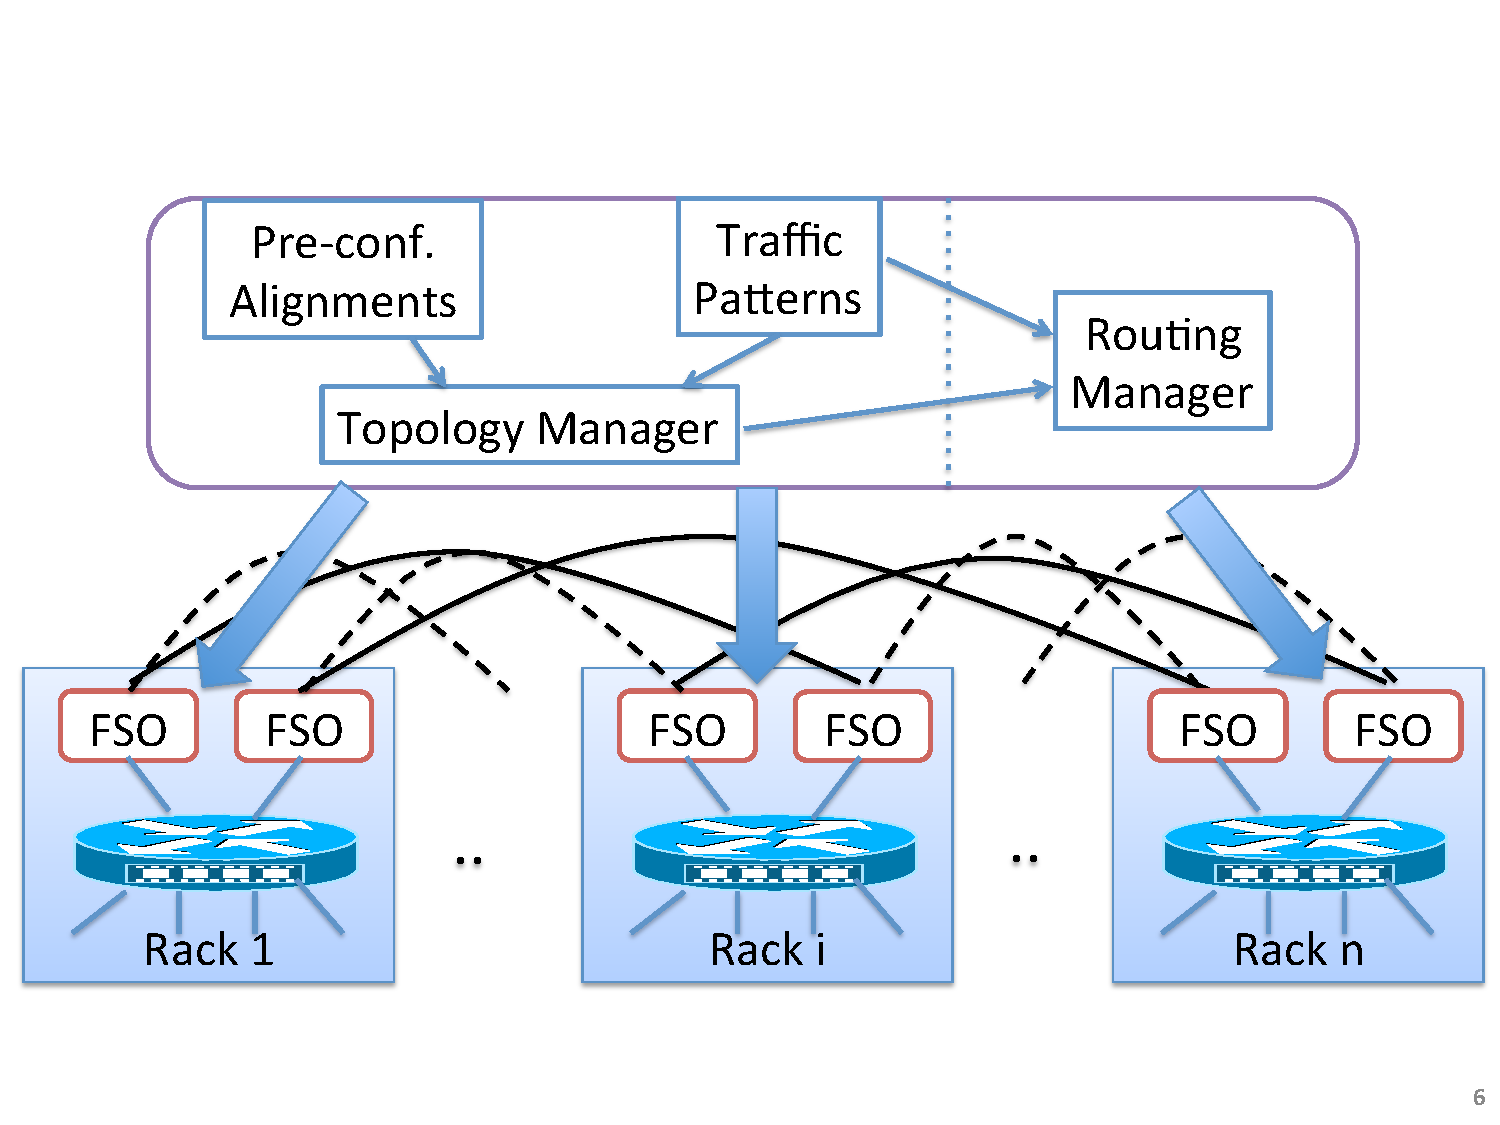
\includegraphics[width=200pt]{Figures/Architecture_New.pdf}
\vspace{-0.4cm} \tightcaption{System overview: The Topology Manager
  decides the set of links to activate and the Routing Manager sets up
  routes for end-to-end flows. At any instant, only one candidate link
  per FSO is active (solid lines). }
\label{fig:arch}
\end{figure}


%We assume there is already a top-of-the-rack (ToR) switch
%that connects the computers in the rack. \blue{There are no
%  higher-level aggregation switches.} \red{Should we give a reason?}

Our vision (see Figure~\ref{fig:arch}) is a \DC network where the ToR
switches are interconnected using FSO devices.  Note that we are not proposing
a fully wireless \DC~\cite{cornell}; our focus is on the
 inter-rack fabric. The FSO transceivers
are placed on top of each rack and aligned to connect, after
reflection from the ceiling mirror, to  devices on other
racks.  %(For simplicity, we assume that each  FSO link 
% is  duplex.) 
 We envision a centralized {\em Topology
Manager} that  dynamically reconfigures the inter-rack
topology\footnote{And hence the title, our conceptual  ``patch panel'' to
reconfigure the topology is ``in the air''!} and the {\em Routing Manager} acts in
concert  with the Topology Manager to setup routing table entries for each
ToR switch to route flows between racks.

Ideally, we would like as many FSO transceivers on each rack and
reconfigure the topology with zero delay.  In practice, this is not
possible. First, given that even a small FSO device is \mbox{3" x 8"},
we can pack only few tens of FSO devices per rack of size \mbox{2' x
  4'}.  Second, existing steering mechanisms are not viable at the
time/costs we envision: mechanical systems take a few seconds and
non-mechanical solutions in the photonics community are still in their
infancy~\cite{elec-survey}.  While miniaturization and reconfiguration
solutions for FSOs will likely improve over the next decade,
our goal here is to work within these constraints and sketch a cost-effective architecture that is
immediately within reach.
% Next we discuss how we can achieve a
%practical reconfigurable architecture working within these constraints.

\subsection{Reconfiguration via Switchable Mirrors}
\label{sec:design-sm}

\begin{figure}[t]
\centering
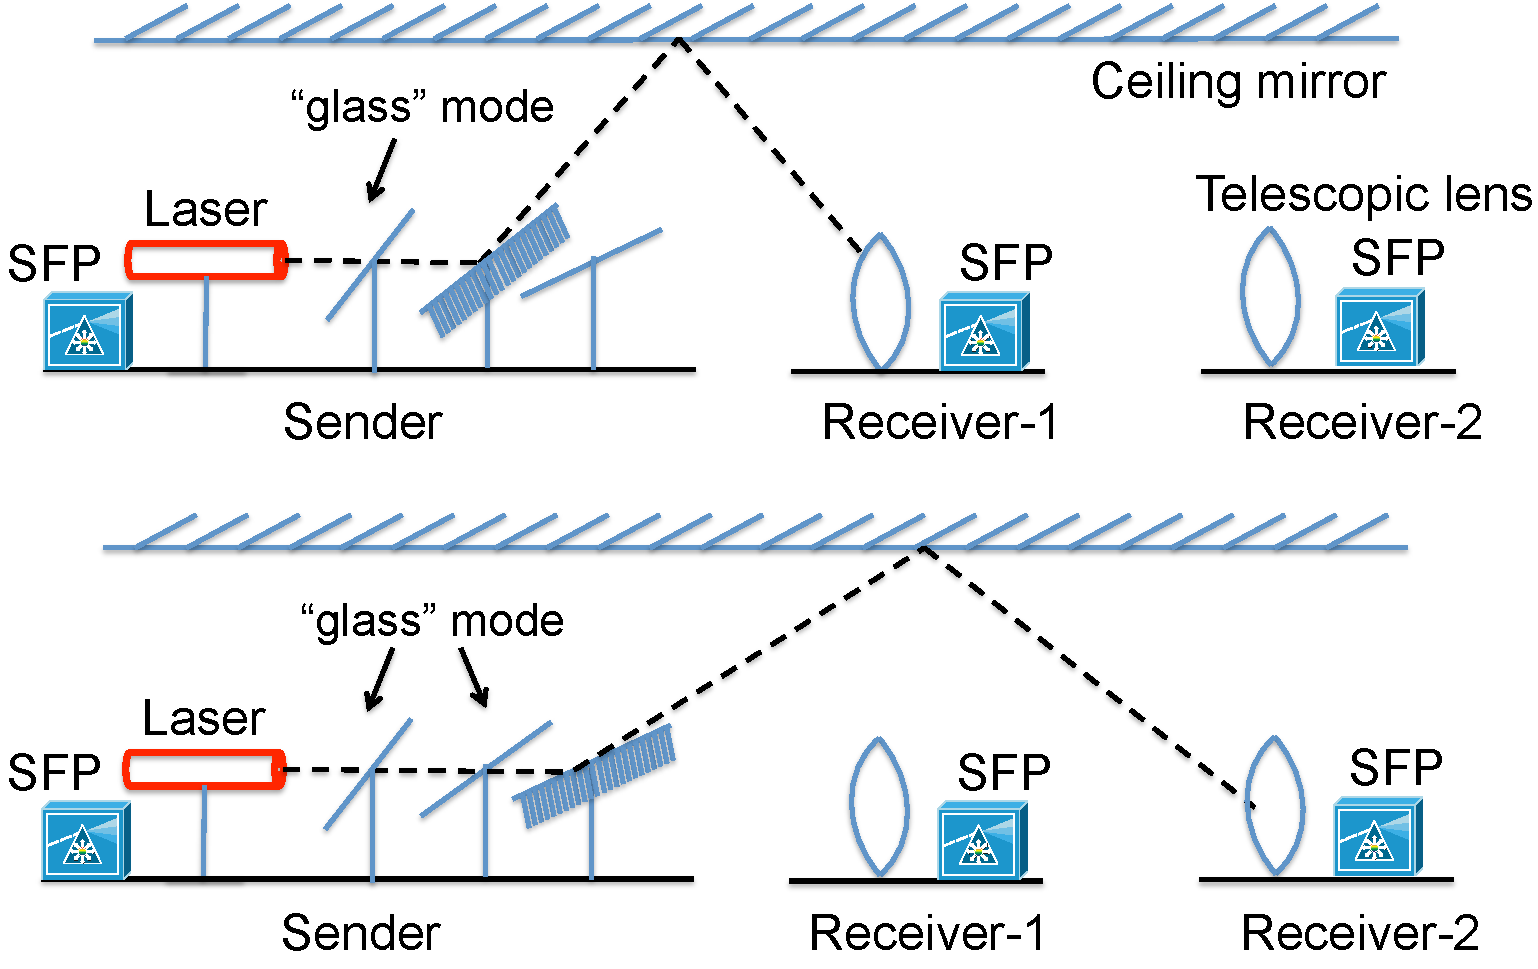
\includegraphics[width=200pt]{Figures/recv-1-2-combined.pdf}
\tightcaption{ In the top half, the second SM is in mirror state, and
  directs the FSO beam to receiver1.  In the bottom half, only the
  third SM is in mirror state, which directs the beam to receiver2.}
\vspace{0.05cm}
\label{fig:link}
\end{figure}
\eat{
Given the delays with mechanical steering and the practical concerns
with the viability of electronic steering, we propose a different
solution for fast reconfiguration.}

We leverage {\em switchable mirrors} (SMs) made from a
special liquid crystal material that can be  electrically controlled
to rapidly switch between  reflection (mirror) and pure transparent
(glass) states~\cite{sm}.  
%The switching latency depends on the size~\cite{sm-size};
%  assuming a \mbox{1'' x 1''} size, the latency is
%about 10-20 msecs.
We equip each FSO device with multiple SMs, and {\em pre-align} the SMs (using
an offline steering assembly) to connect to an FSO on a different rack. As
shown in Figure~\ref{fig:link}, a link is established by keeping one of the SMs
in mirror state and the other SMs in that FSO in transparent state.  (An
analogous configuration exists at the other end to create a duplex link, but not shown.) In
essence, the pre-alignments of the SMs  yield a set of {\em candidate} links.
At any instant, only one  of the candidate links is {\em active} per FSO 
based on the SMs' state. (See~Figure~\ref{fig:arch}.) 
 When manufactured at scale, each small-size SM 
 will cost $<$ \$5~\cite{sm-personal}.


\para{Proof-of-concept:} We built a proof-of-concept prototype to
evaluate the viability of switchable mirrors. As a pragmatic choice, we use
off-the-shelf components: (1) LightPointe FlightStrata G Optical Gigabit
Links~\cite{lightpointe}; (2) A \mbox{12'' x 15''} switchable mirror (SM) from
Kentoptronics~\cite{sm} tuned for IR spectrum; and (3) normal
mirrors.\footnote{The prototype is larger than the
 \mbox{3'' x 8''} form factor we envision as 
 the equipment is designed  for
outdoor use.}
  % We aligned the FSO devices such that (i) FSO devices 1 and 2 form a link when
 %the SM is in its mirror state, and (ii) FSOs 1 and 3 form a link when the SM is
%in its transparent state.  
 We found that the switching latency of the SM was around 250~ms.
Because the switching latency is proportional to the SM's surface area~\cite{sm-size}, we
conservatively estimate a 20~ms latency for the (\mbox{1'' x 1''}) SM we
propose to use. We also confirmed that the FSO beam is reflected from
conventional mirrors with negligible loss and achieves full achievable bitrate.

\para{Degree of Reconfigurability.}  In practice, size constraints will likely
limit the number of SMs per FSO device. In our current architecture,
we conservatively assume that it is feasible to add 5-10 SMs on an FSO
device, with the overall device still $\approx$ \mbox{3'' x 8''} in
size.  Our design using a finite number of SMs provides a 
sufficient degree of reconfigurability (i.e., activating some subset
of candidate links by switching states of SMs) at fast
timescales.\footnote{Even though mechanically steering the SMs/FSOs
  provides full reconfigurability, this takes few seconds or
  minutes.}
   \blue{Reconfiguration using SMs effectively removes  the
  need to {\em realign} the FSO devices. Furthermore, since the 
  pre-configuration is done relatively infrequently, it need not
  be achieved at a fast timescale.}

%In doing so, this design addresses a potential 
% concern with FSO deployment in \DCs, namely alignment.} 
% This address one of the biggest
%  hindrances to viability of FSO-based designs in datacenters.}
  
Our remaining tasks are: (1) Choose an appropriate {\em
  pre-configured} topology (i.e., candidate links defined by the SMs'
pre-alignments); and (2) Design dynamic reconfiguration \\ mechanisms
(i.e., activating select links) to adapt to traffic patterns.  We
discuss these next.

\subsection{Pre-configured Topology}  
\label{sec:pre-conf}

Our goal in this paper is not to design an optimal pre-configuration
topology. Rather, we want to demonstrate the potential benefits of an
FSO-based inter-rack design.  To this end, we discuss two promising
starting points. 


% VS: this really  comes out of nowhere .. dropping this for now
%\blue{We note that, unlike other
%  works~\cite{cthrough,helios,3db}, we don't enforce a requirement
%  that our pre-configured topology contain a base {\em static}
%  subtopology, but instead ensure (see \S\ref{sec:reconfig}) that at
 % {\em all} times there is an underlying (perhaps, changing) connected
 % topology.}

\para{Regular Random Graphs:} Recent work shows that random regular
graphs provide bandwidth and latency comparable to structured
topologies~\cite{jellyfish}. \blue{Furthermore,  a random graph  is naturally amenable
  to  incremental expandability.}  If each FSO is equipped with $k$ SMs,
then we create a $k$-regular random graph over the FSOs by aligning
the SMs appropriately.  In fact, FSOs act as an enabler to leverage
the benefits of such structures by eliminating  potential
concerns about the wiring complexity and mis-wiring (see~\cite{jellyfish}, Section~6).
% Second, by providing a mechanism
%to ``re-randomize'' the network, it alleviates fears that a specific
%graph instance may be sub-optimal within the space of random
%topologies. 

%I'm keeping the hypercubes for now, because of the low-k high-n argument.

\para{Hypercube + Random Links:} \cam{If the node degree is low relative to
 the number of racks,  a random graph may not have good connectivity.
This might become relevant in the regimes we are considering---degree is a few tens, and number of racks/nodes may be a few hundred.}  
Thus, we consider
an alternative topology where we use some SMs to construct a
``baseline'' topology that guarantees connectivity properties, and
align the remaining SMs randomly.

We believe that a hypercube is a suitable  baseline
topology for three reasons: (1) it uses a small number of links and
 leaves many candidate random links; (2) it has a small
diameter ($\log n$ for $n$ racks); and (3) it has high bisection
bandwidth ($n/2$ over $n$ racks).  Furthermore, the performance of a
hypercube can be improved by adding {\em diagonal} edges which connect
each node to its ``complement''; these ``short-cuts'' halve the
diameter (proof omitted).  We also conjecture based on simulations 
 that the diagonals also improve (roughly double) the
bisection bandwidth.

%\green{As an example, in a datacenter with 512 racks, we
%   use 10 SMs from different FSOs on each rack to form this
%  extended hypercube (9 for hypercube and 1 for extra diagonal); we
%  align the remaining SMs to create random inter-rack links.}

\subsection{Dynamic Reconfiguration} 
\label{sec:dyn}
 We have two sub-tasks here. First,  given a pre-configured topology, we
need to choose a suitable set of active links out of the candidate links
depending on current traffic patterns. Second,  unlike prior hybrid
architectures~\cite{cthru,helios,3db}),  our network does
not contain a fixed wired backbone.  Thus, one potential concern is that
reconfigurations \blue{(by changing the states of SMs)} may result in
transient connectivity problems.  We sketch solutions to address each
challenge.

\para{Reconfiguration Strategy:}  Designing an optimal strategy is
challenging because \DC workloads are diverse and hard to
predict~\cite{vl2}. Our goal is not to seek optimal solutions, but  a
feasible yet performant architecture. To this end, we use a heuristic based on 
 prior  work~\cite{helios,mahout}:

\begin{packeditemize}
\item Short flows (e.g., $\leq$ 1MB~\cite{helios,mahout}) are
  routed along the shortest path  formed by currently
  active links.

\item For large flows (i.e., $>$ 1MB), we evaluate if activating 
  some link(s) can provide higher throughput than routing it
  over the current network.   In our current
  design,  we only activate links that yield a
  shorter and/or less-congested paths to the destination.
\end{packeditemize}


We can extend this along several dimensions as  discussed in
\Section\ref{sec:future}.  As such,  the quantitative benefits  we show 
in \S\ref{sec:perf} can be viewed as an immediately achievable lower bound
of the benefits our vision can offer.

\para{Lossless Reconfiguration.} Given the finite latency involved in
changing SM states, we need to ensure that we don't drop packets or disrupt the
flow of latency-sensitive packets during this transition. At a high-level, we
achieve this by ensuring that  there is always a ``valid'' routing table 
 even during reconfigurations;  i.e.,
each entry corresponds to an active link.  To see the intuition behind our
approach, we start with a simple reconfiguration to activate a single edge
$(x,y)$, between FSO devices $x$ and $y$,
 and  deactivating the currently active links 
 $(x,w)$ and $(y,z)$. The key here is in the ordering of
the steps---we remove routes before deactivating links and add routes only
after activation is complete as shown below:

%To guarantee a valid routing table at all times, we use
%the following sequence of steps. 

%
\begin{packedenumerate}
\item
Avoid this reconfiguration, if deleting active links of the type
$(x,w)$ or $(y,z)$ (to free the FSOs $x$ and $y$) will disconnect the
network.\footnote{To ensure that a reconfiguration request is {\em
    never} rejected, we can use some of the FSOs per rack to
  implement a static connected graph (e.g., ring)   and never change these
  links.}

\item
Update the routing table to reflect removal of  links $(x,w)$
and $(y,z)$.

\item
Switch the states of appropriate SMs to: (i) deactivate  links
$(x,w)$ and $(y,z)$, and (ii) activate the link $(x,y)$. Note that
this step can take $\approx$ 20~ms.

\item
{\em After} completion of the above step, update the routing table to
reflect addition of link $(x,y)$.
\end{packedenumerate}

%Since the reconfigurations occur in response to changing traffic
%across the network,
We may need to handle multiple potential reconfigurations that occur
almost simultaneously in response to traffic changes. Multiple
reconfiguration can be handled in one of three ways: (i) one at a
time, (ii) in batches (i.e., queue and combine them into a single
reconfiguration); and (iii) execute each reconfiguration individually
but {\em concurrently}. The first two options can be inefficient as
large flows wait until the desired link(s) become
available. We believe that the third option can be achieved by a careful
implementation of step \#1 above. 

% (We skip the details for brevity.)

\eat{ Since the reconfigurations happen in response to changing
  traffic across the network, reconfiguration requests at any
  time. For better performance, these reconfiguration request must be
  handled ``concurrently,'' i.e., {\em not} one a time (since each
  request could take tens of milliseconds).
%
However, concurrent handling of request could result in an
``inconsistent'' routing table. But, it can be shown (we omit the
details) that if the first two steps of the above process are
implemented as one {\em atomic} step (i.e., not interleaved with any
step of other requests), then multiple {\tt activation} requests can
be handled concurrently while still guaranteeing a valid routing table
at all times.  }

%Now, to ensure that the {\tt activation} request is {\em never} rejected,
%we can use some of the FSOs on each rack to implement a {\em static} base 
%topology. E.g., we can use one FSO on each rack to create a ring topology
%connecting all the racks; the SMs in these FSOs (one per rack) are never
%switched to keep the ring topology static. 

%% 1 page
\section{Performance Benefits}
\label{sec:perf}

%We now present some initial benchmarks and results to justify the
%feasibility of our vision.
In this section, we use a custom simulator to compare the
performance of our FSO-based architecture(s) against state-of-art  \DC
designs.   As a representative point, we consider a \DC with 24,576
machines organized into 512 racks of 48 machines. Our results are
qualitatively similar for other configurations.


\begin{table}[t]
\begin{small}
\begin{center}
\begin{tabular}{c|c|c}
%\hline
Architecture & Cost (\$) & Effective per-server throughput \\   \hline % \hline
FSO-based (16,5) & 18.1M  & 1.7 Gbps\\    %\hline
3D Beamforming & 17.1M  & 1.1 Gbps\\% \hline
Fattree/Jellyfish 1Gbps & 13M & 1 Gbps\\%   \hline
Fattree/Jellyfish 2 Gbps & 26M  & 2 Gbps \\ \hline
FSO (48,10) & 37.8M  & 8.5 Gbps \\ %\\   \hline
Fattree/Jellyfish 10Gbps & 57M  & 10 Gbps%\\   \hline
\end{tabular}
\end{center}
\end{small}
\vspace{-0.3cm}
\tightcaption{Cost-performance tradeoffs for 512 racks with 48 machines/rack:
 The FSO designs are specified by (\#FSOs, \#SMs/FSO).}
\vspace{-0.3cm}
\label{table:cost}
\end{table}

\para{Candidate Architectures and Costs.}
 The specific architectures we consider 
are:\footnote{We don't consider the all-wireless architecture
of~\cite{cornell} because  it has
worse cost-performance tradeoffs relative to the below
architectures; e.g., for 24k machines, it costs $\approx 50M$ (based on \$1k for a 60GHz radio) 
but only achieves 300-400 Mbps per-server and has an
average/max. hop-count of about 10/100~\cite{cornell}.}

\begin{packeditemize}
\item {\bf Fat-tree~\cite{fattree}:} We consider
   1Gbps and 2Gbps bisection-bandwidth FatTree networks. A
  2Gbps network is essentially two 1Gbps networks put together.

\item {\bf Jellyfish~\cite{jellyfish}:} We construct wired random
graphs~\cite{jellyfish} and similar to FatTree, we consider both 1 and 2~Gbps
architectures.

\item {\bf 3D-Beamforming~\cite{3db}:} We use a wired 1Gbps
  bisection-bandwidth network augmented with eight 60GHz wireless
  radios per rack~\cite{3db}. We conservatively assume 0.01s antenna
  rotational delay (lower bound from~\cite{3db}), no interference, and
  a 1-10~Gbps bandwidth for wireless links based on inter-rack
  distances~\cite{3db}.

\item {\bf FSO-based designs:} We use two pre-configured topologies
  (\S\ref{sec:pre-conf}): (1) {\tt Random} and (2) {\tt Hypercube+}.
  We use a 64-port 10Gb ToR switch~\cite{64switch}; 48 ports
  connect to machines and 16 ports  to FSO devices.
  Each FSO link is 10~Gbps, since we use 10Gbps optical SFPs as
  our cost basis.  We assume each FSO device has 5 SMs,
  with a switching latency of 20~ms.
%and  also study   the effect of varying this, a SM switching latency of 20~ms.
%\blue{Based on our experiment, we    use a switching latency of 20 msec.}
\end{packeditemize}

Ideally, we want to compare architectures by normalizing their cost.
Unfortunately, some architectures (e.g., Fat-tree, {\tt Hypercube+})
do not admit a continuous spectrum of cost-performance
tradeoffs. Further, some of these cost estimates are moving targets.
As such, we pick configurations where the costs are roughly comparable
based on estimates we obtain as discussed below.

We assume that a 64-port 10Gb ToR switch for the FSO designs costs
\$27K: \$11K for the bare switch~\cite{64switch}, and \$16K for 64
10Gbps optical SFP+ transceivers at \$250 each~\cite{sfp}. We assume
that a 48-port 1Gb switch costs \$5000~\cite{48-switch-cost}, and each
60GHz radio costs \$1000. From \S\ref{sec:fso}, each FSO device costs
an additional $\approx$ \$500 with \$5 for a small-size SM, when
manufactured at scale~\cite{sm-personal}.  We assume ceiling mirrors
(for FSO and 3D-beamforming) have negligible cost and we
conservatively ignore cabling costs for the wired architectures. Given
the above assumptions, Table~\ref{table:cost} summarizes the costs.
Here, Fat-tree/Jellyfish 1Gbps use  2600 48-port 1Gb switches. We
see that FSO-based designs roughly fall between the 1~Gbps and 2~Gbps
wired architectures. As additional points of reference, the table also
shows 10~Gbps architectures for FSO and Fat-tree (discussed later).

%\footnote{We do
 % not have access to real datacenter workloads and the public ones
  % that exist do not map data sources to rack locations.}

\begin{figure}[t]
\begin{center}
\subfloat[Uniform]
{
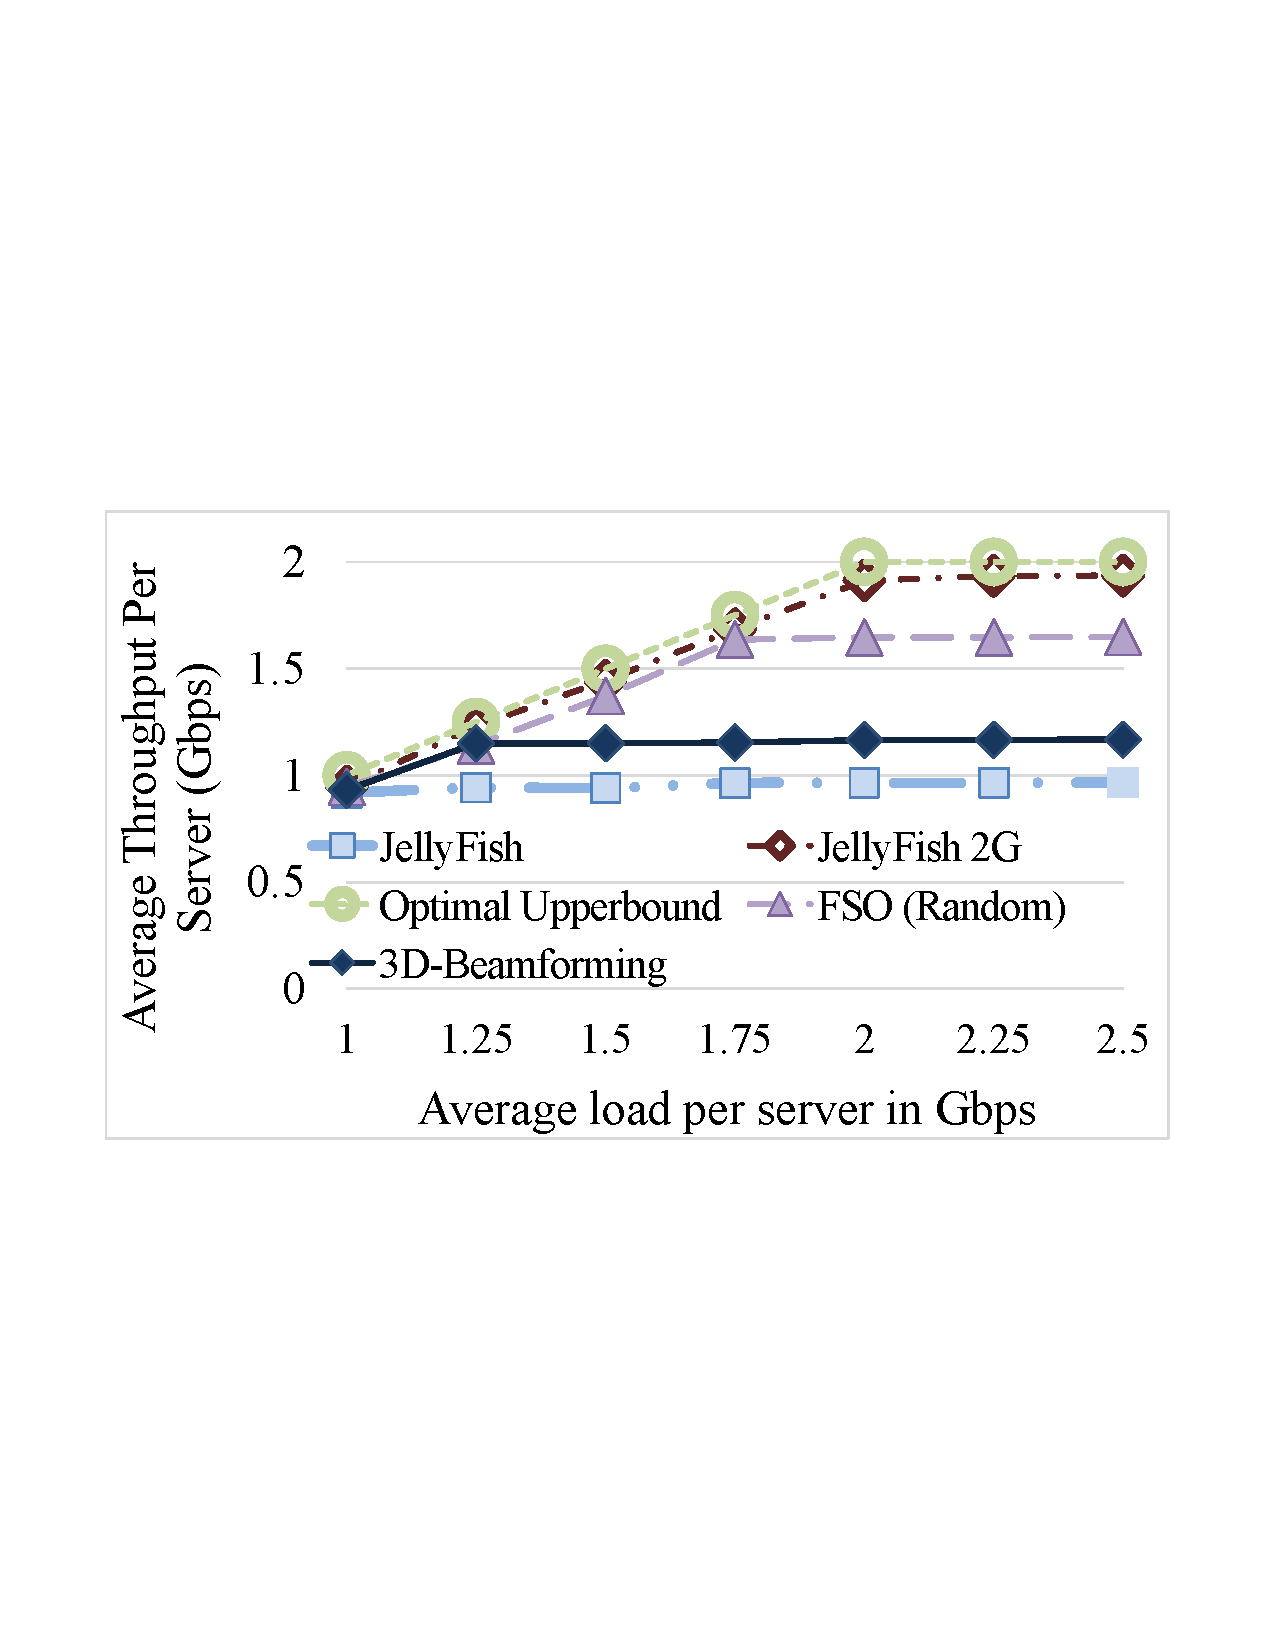
\includegraphics[width=180pt]{Figures/NewFigures/NormalTraffic.pdf}
} \\ \vspace{-0.3cm}
\subfloat[Hotspot]
{
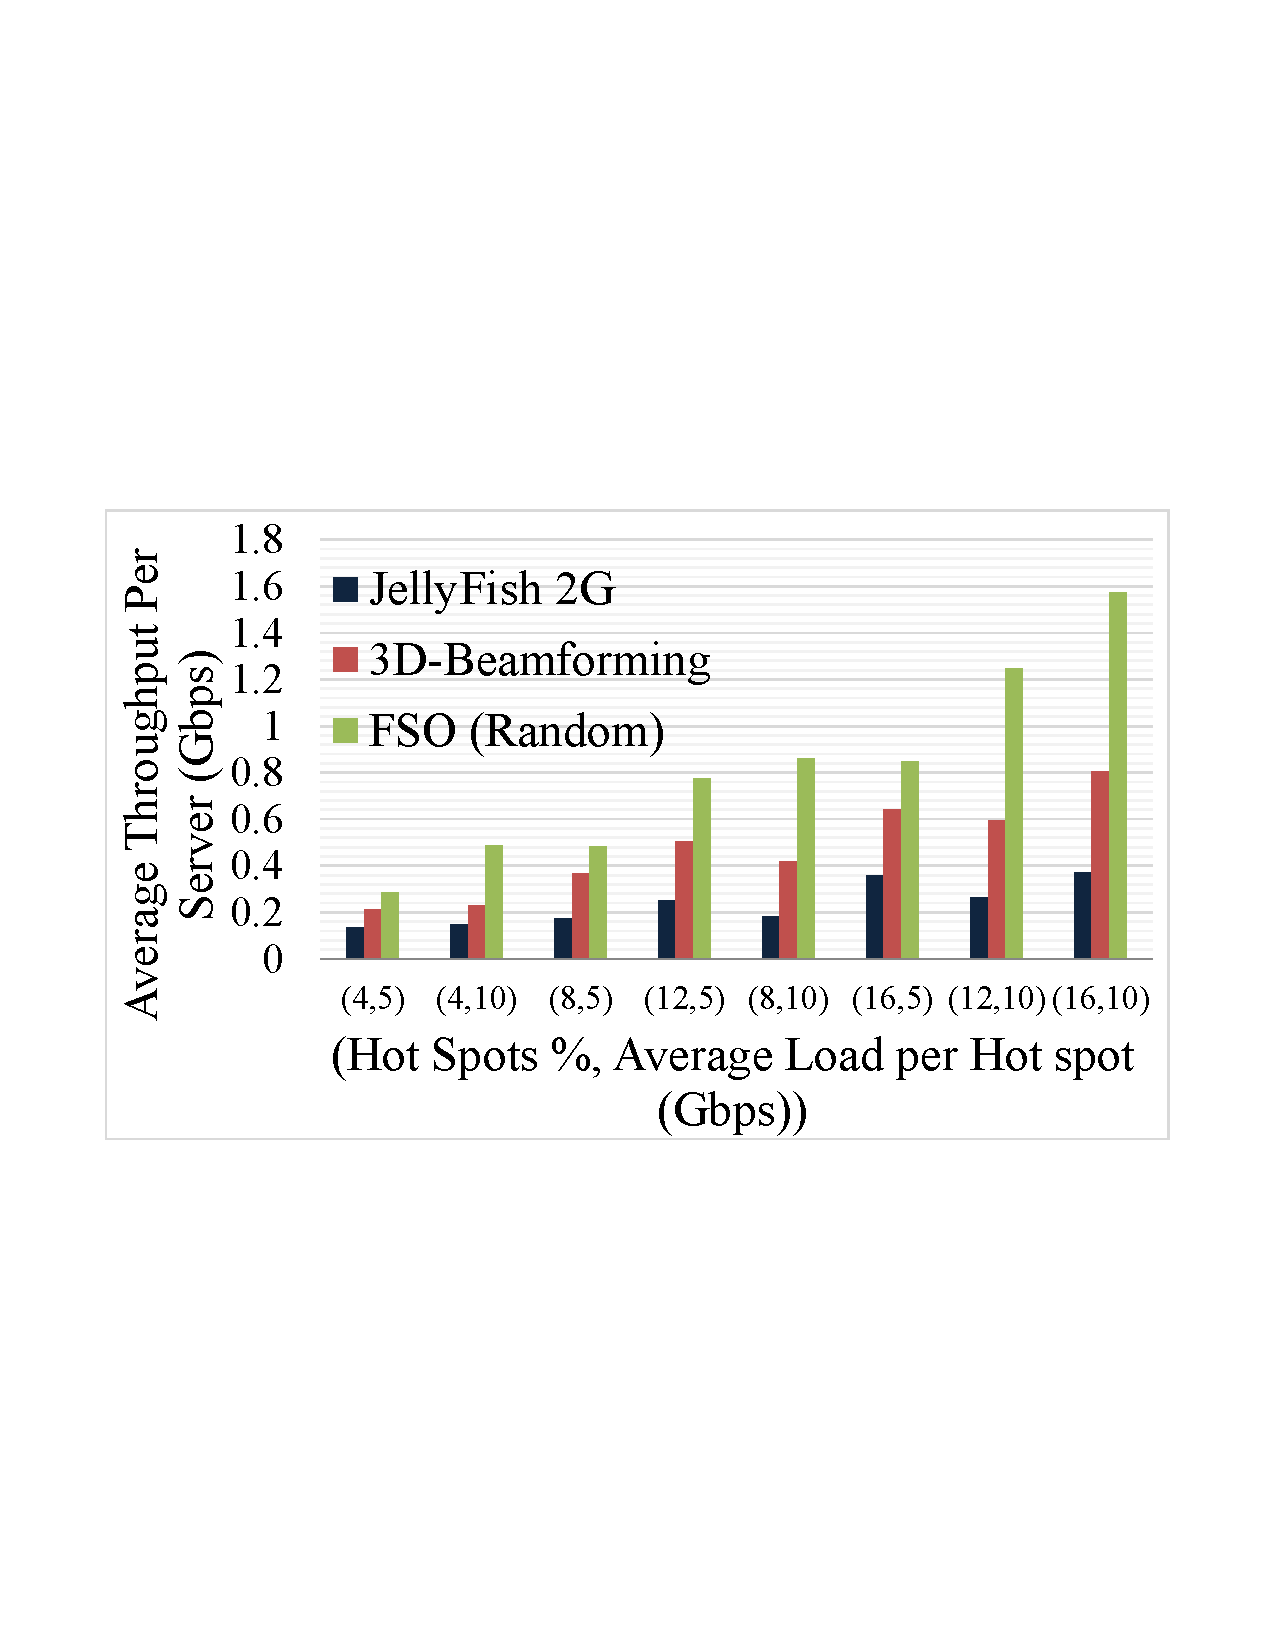
\includegraphics[width=180pt]{Figures/NewFigures/Hotspots.pdf}
}
\end{center}
\vspace{-0.3cm} \tightcaption{Average per-server throughput for the
  {\tt Uniform} and {\tt HotSpot} workloads.  The
  $x$-axis shows the average load per server which is a 
  product of arrival-rate (per pair), number of servers (512),
  and average flow size. The result for Hypercube+  is identical 
 to Random and the result for Fat-tree is identical to Jellyfish 
 and are not shown.}
\vspace{-0.3cm}
\label{fig:tput}
\end{figure}

\para{Simulation Setup.} For scalability, we consider 
   a flow-level simulation using a fluid model, and do not model 
 packet-level or TCP effects. 
% assuming} the buffer queue
%of each switch to be bounded (400MB) with the ``overflow'' packets
%being dropped.
 We use synthetic traffic models based on
prior measurement studies as follows~\cite{vl2,3db}.  We consider a
{\em baseline} workload where, for each pair of machines, flows arrive
independently based on a Poisson distribution with a {\em
  arrival-rate} $\lambda$/s, with the flow size distribution
measurements from production \DCs~\cite{vl2}.  We refer to
this as the {\tt Uniform} workload.  Prior studies have observed
hotspots between pairs of racks~\cite{vl2}; thus we consider the {\tt
  Hotspot} model where in addition to the {\tt Uniform} baseline, we
use a higher arrival-rate $\lambda_2$ and a fixed flow-size of 128MB
for a subset of machines chosen as follows~\cite{3db}. We randomly
pick $x$\% of machines, and for each one of them, we pick $x/2$\% of
machines as their destinations with a slight bias~\cite{3db}; we vary
$\lambda_2$ and $x$ in our simulations.  

\para{Throughput and Latency.}  Figure~\ref{fig:tput}(a), shows the average
per-server throughput for the {\tt Uniform} workload.  We observed that
Jellyfish and Fat-Tree architectures are nearly identical  and the two
FSO-based architectures (Random and Hypercube+) also have the same performance.
For ease of presentation,  we omit  plots for Fat-Tree and Hypercube+.

\begin{figure}[t]
\vspace{-0.3cm}
\begin{center}
%\begin{tabular}{cc}
\subfloat[Vary \#SMs]
{
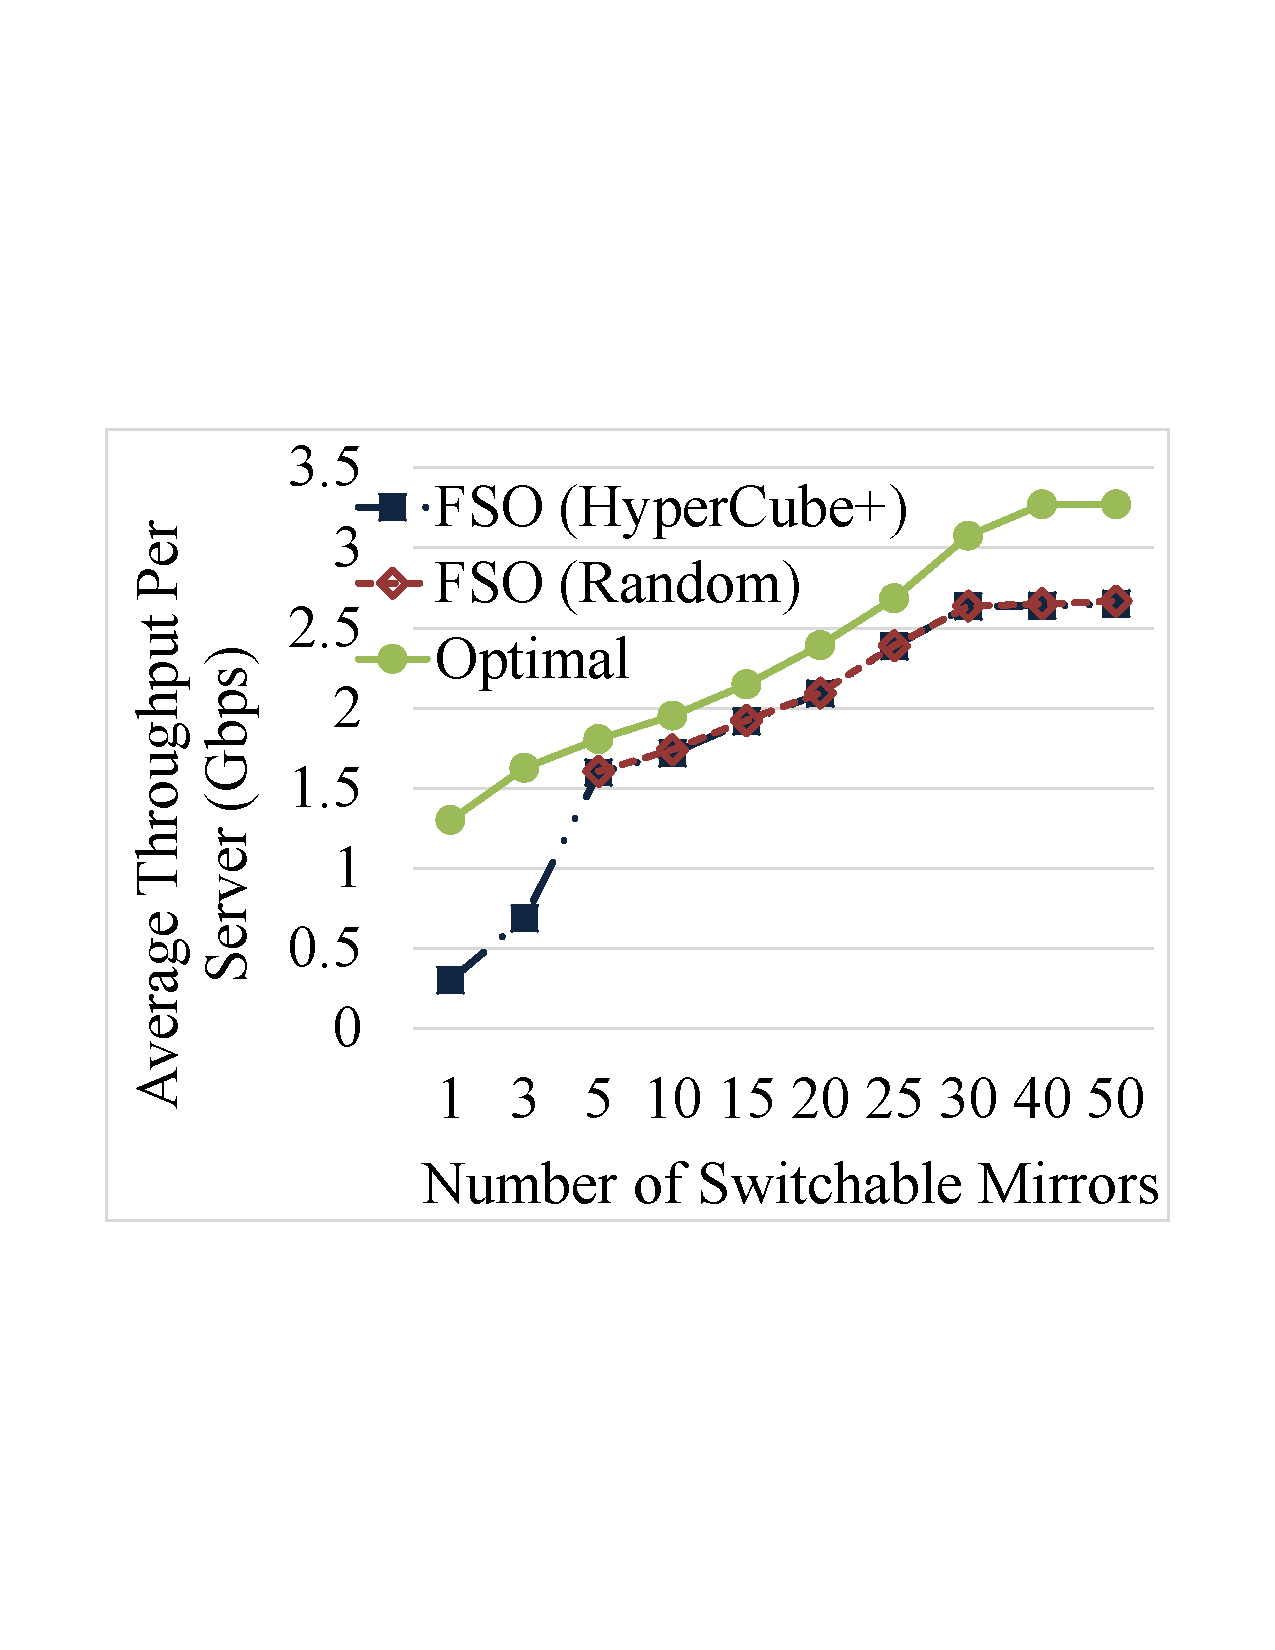
\includegraphics[width=0.22\textwidth]{Figures/NewFigures/Mirrors.pdf}
}
\subfloat[Vary \#FSOs]
{
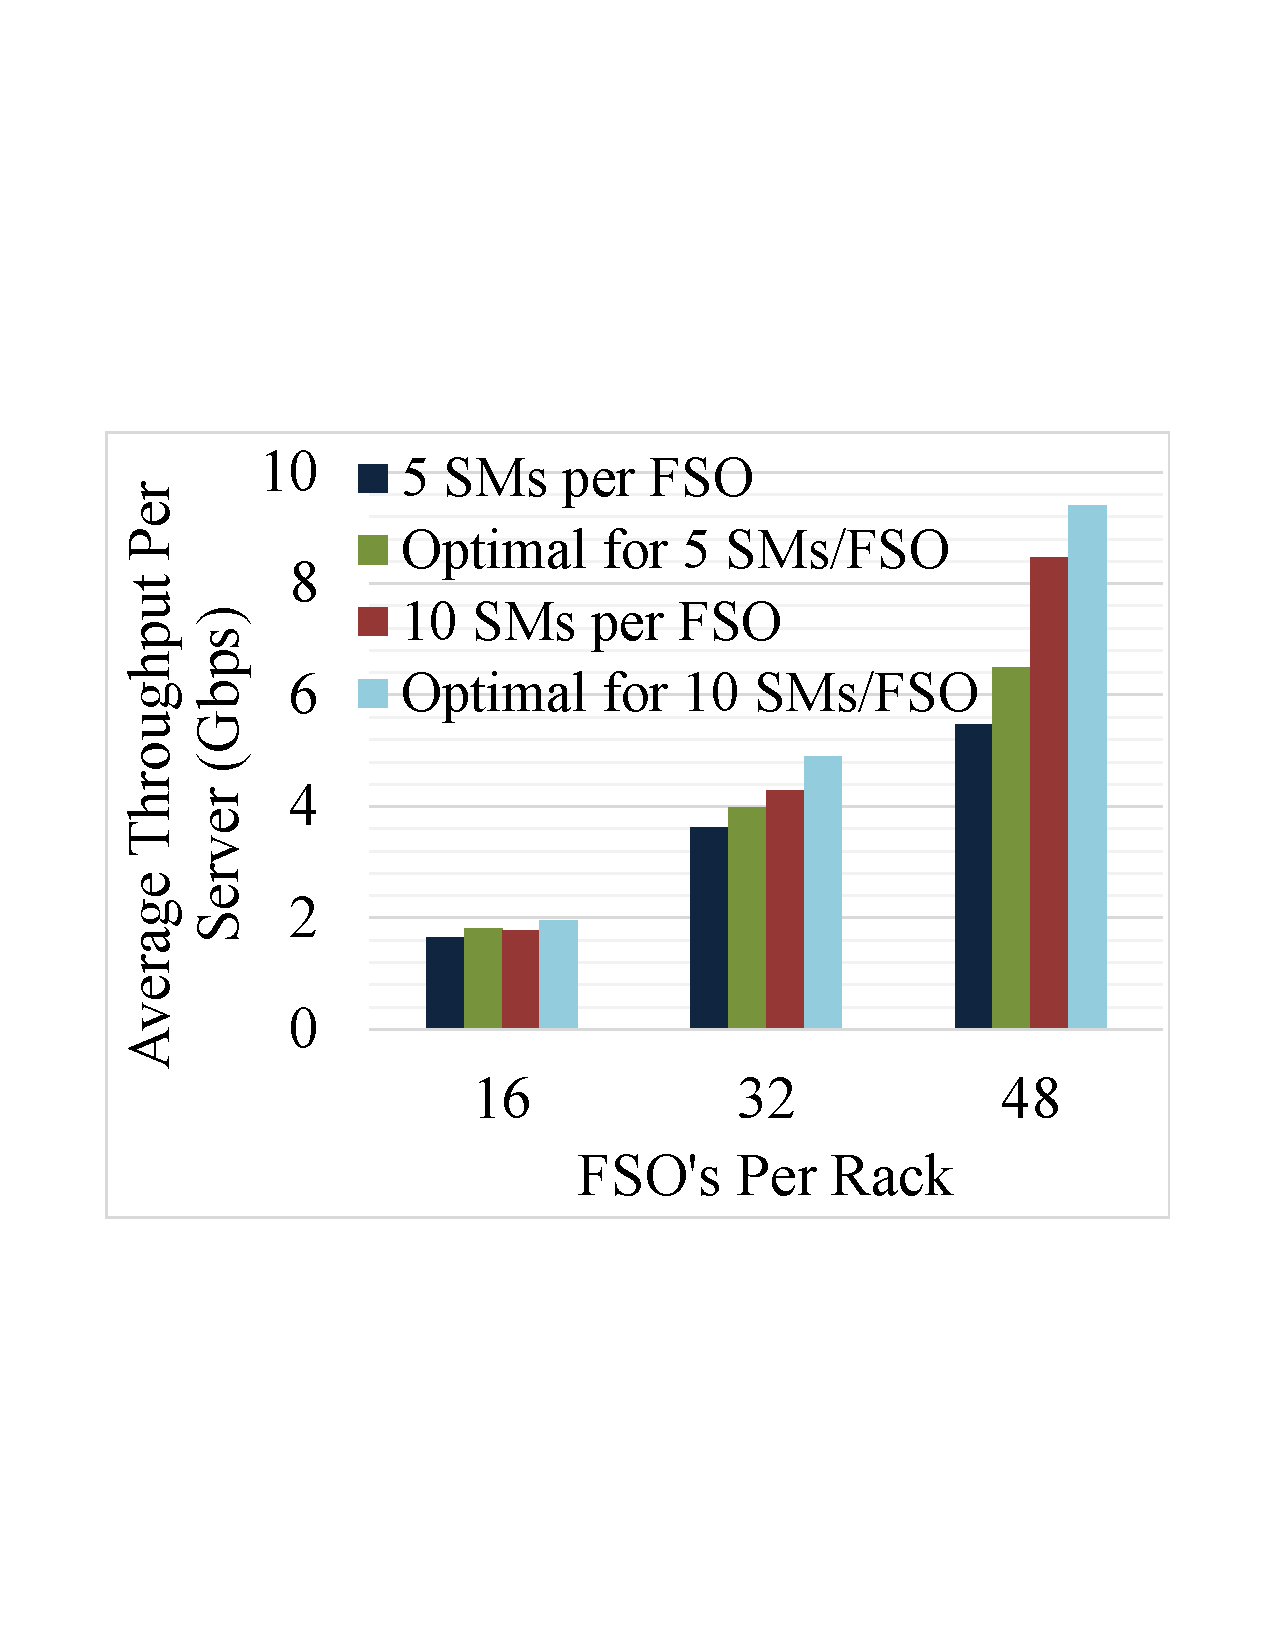
\includegraphics[width=0.22\textwidth]{Figures/NewFigures/FSOMirrors.pdf}
}
%\end{tabular}
\end{center}
\vspace{-0.3cm}
\tightcaption{Sensitivity analysis,  varying number of FSOs and number of SMs using
 the baseline {\tt Uniform} workload}
% Average per-server throughput for various
%  configurations at {\em saturated} loads. (a) Varying number of SMs
%  per FSO, with 16 FSO per rack. (b) Varying number of FSOs per rack,
%  with 5 or 10 SMs per FSO.  Both experiments use a {\tt Uniform}
%  traffic, with an average server load of 5Gbps and 20Gbps
 % respectively.}
\label{fig:sms}
\end{figure}

We see that FSO-based architectures provides 1.7Gbps of average
throughput per server, which is significantly higher than 1Gbps
Jellyfish/Fattree and 3D-Beamforming, but slightly lower than the
2Gbps Jellyfish/Fattree.  As a point of reference, we compute an
upper bound on the {\em optimal} throughput achievable with FSOs. Given
a configuration of \# FSOs per rack and \# SMs per FSO, we compute
this bound by estimating the minimum possible average shortest-path
length; we omit the details due to space limitations. We see that our
design performs quite close to the upper-bound of $\approx$ 2Gbps.

For the {\tt HotSpots} workload in Figure~\ref{fig:tput}(b), as
in~\cite{3db} we use a low baseline load of 0.1Gbps average load per
server.\footnote{We also tried other baseline loads. FSO
  outperforms other solutions under all scenarios, but the relative gain
  decreases at higher load as there is less scope for
  improvement.}  We consider different configurations for the number
of hotspots and intensity (i.e., $x\%$, average load per hotspot) as
shown. First, we see that all flexible architectures (FSO-based and
3D-Beamforming) outperform the static Jellyfish (and Fat-Tree) 2Gbps
designs.  Second, the FSO-based design outperforms 3D-beamforming by
large margin (30 to 100\%).

We also measured the latency in terms of inter-rack hops per-packet.
The average, 95\%ile, and max latency for FSO-based proposals were
2.5, 6, and 12 hops respectively (not shown). In comparison, the
corresponding numbers for Fat-tree and Jellyfish are 3.9,4,4 and
 2.5, 3, 5 hops respectively. We see that in the common case, FSOs
provide low latency, but in some very rare cases we incur longer
paths.

% (For reference, the 95\%ile latency for FSO is 6 hops which is
% comparable to the max for others).

% \vyas{is this inter rack or inter machine .. also show fattree or jellyfoish as point of reference}

\para{Sensitivity Analysis.} The previous results consider a fixed number of
FSOs per rack and SMs per FSO device. In Figure~\ref{fig:sms}, we vary (a) the
number of SMs keeping the number of FSOs at 16/rack, and (b) the number of
FSOs per rack for 5 and 10 SMs/FSO.  (We do not show  {\tt Random} for less
than 5 SMs, since it does not form a connected graph.) First, we see that the
effective per-server bandwidth increases with the increase in SMs, but
saturates at around 30 SMs per rack (when we almost get a complete candidate
graph).  Second, the configuration of 48 FSOs with 10 SMs provides almost
8.5Gbps. 

Given our current size estimates, it is actually feasible to place 48
FSOs on each rack; the total cost of this architecture is $\approx$
\$38M.  We estimate this assuming a 96-port 10Gb switch (hypothetically)
costs \$49k (= \$25k for the  switch + cost for 96 SFP+ modules at \$250
each).  In comparison, a 10Gbps Fat-tree architecture would
(conservatively) cost around \$57M assuming each 48-port 10Gb switch
costs \$22k (= \$10k~\cite{48-10-switch} + cost for 48 SFP+ modules).

%% 1 page
\section{Discussion} 
\label{sec:future}

%Further Challenges}

%\green{Before we conclude, we discuss other research challenges and opportunities
% that  our  vision of a flexible FSO-based datacenter network  introduces. }

\para{Rethinking Metrics of Goodness.}  Traditional  metrics  such as  bisection bandwidth and diameter largely reflect a
{\em static} perspective of the topology. For the types of flexible networks we
envision, we need to  rethink these metrics; e.g., 
we  need a notion of  {\em dynamic} bisection bandwidth  based on the best achievable
  bandwidth by some {\em realizable} topology for a given 
network partition.

\para{Optimal Topologies.} Given new dynamic performance indices, we need to
reason about the  pre-configured alignment of SMs that optimizes these
metrics. While the random and extended hypercube designs work well, we do not
know if these are provably (near-)optimal.  Furthermore, choosing an optimal
run-time topology is effectively an  online optimization problem---given a
pre-configured topology, current configuration and traffic patterns, what is
the best way to reconfigure the network?  What makes this  challenging is that
even the offline version of this problem is intractable. 
 
%Here, the switching latency should be taken into consideration. We note that
%even the {\em offline} version of the problem is computationally intractable.

\para{FSOs for Modularized Data centers.} While our current work
focuses on the inter-rack fabric, FSOs might also be useful for
 containerized architectures~\cite{helios}.  This context
introduces new challenges and opportunities.  Specifically, a ceiling
mirror is not feasible in outdoor scenarios and we need other
mechanisms (e.g., vertically steerable FSOs?) for line-of-sight. At
the same time, the coarser aggregation may permit higher switching
 latencies and thus be amenable to slower (mechanical) steering
mechanisms that can provide full reconfigurability.

\eat{
This could imply that we may be less concerned by the cost of
individual FSOs (as there are fewer).  Furthermore, the traffic
patterns may be more predictable, and thus amenable to other steering
technologies (see below).}

\para{Multipath and Traffic Engineering.}  We could further improve
the performance using multi-path TCP~\cite{multipathtcp} or better traffic
engineering~\cite{thorup}. We posit that multi-path TCP has 
natural synergies with reconfigurability as it can  
alleviate transient congestion and connectivity issues.


%how does topology  design affect these?

%Our use of SMs with a pre-configured
%topology represents a practical FSO architecture that can be
%cost-effectively implemented given today's commercially available
%technologies. That said,



%\para{More Degrees of Freedom.}  Future FSO designs may provide more degrees of
%freedom: mechanical and non-mechanical steering of SMs and  lasers~\cite{elec-survey}.  An 
% interesting question is to  match the
%timescales of reconfiguration each mechanism offers vs.\ the predictability 
%of traffic patterns; e.g., planned  VM migrations 
% may be amenable to slower steering options.

% and the
%  dynamicity of the traffic.} \red{Can be made clearer.}

\para{Other Benefits.} In addition to the quantitative benefits we
explored, FSO-based flexible architectures also offer other qualitative
advantages. First, by acting as an enabler for new topologies, it naturally
inherits the  properties  they provide; e.g., random graphs offer incremental
expandability~\cite{jellyfish}. Second, selectively disabling links may also
decrease energy costs~\cite{elastictree-nsdi10}.  Furthermore, by eliminating
the wired infrastructure, FSOs can potentially reduce  cooling costs by 
 avoiding  problems due to airflow  obstruction~\cite{airflow}.

%and power (e.g.,  by eliminating aggregation switches) costs.
 
%  VS: dont know what navid had .. but here are a couple ones:
	% http://www.cisco.com/en/US/solutions/collateral/ns340/ns517/ns224/ns783/white_paper_c11-473501.html 
	%http://www.mm4m.net/library/Avoidable_Mistakes_that_Compromise_Cooling_Perfomance.pdf

%  power/cooling, cabling cost 


%ese future designs will require novel
%techniques for optimal topology design.

%\vyas{Exploring nonmechanical steering platforms goes here}


%% 0.25
\section{Conclusions}
\label{sec:conc}
We explored an FSO-based inter-rack fabric for data centers, a solution whose
benefits have been suggested~\cite{us-patent,hotnets09scribe}, but has
received little attention in depth. We showed that FSOs can be viable with the
extensions we propose (e.g., switchable mirrors and pre-configured
topologies).  Our evaluations show that FSO-based designs offer good
cost vs.\ performance tradeoffs (Table~\ref{table:cost}) w.r.t.\ state-of-art
solutions; e.g., close to 9~Gbps bisection bandwidth at much less cost
compared to a Fat-tree, and 90\% of the performance for 2~Gbps fat-tree at
70\% of the cost.  We note that these benefits only represent an early
starting point---miniaturization and commoditization will further improve
the cost-performance tradeoffs and flexibility that FSO-based designs can
offer.



%further remove many of the
%cost/size constraints and enable \blue{greater flexibility} for
%FSO-based datacenters.

\eat{We are currently exploring several dimensions to turn this
  initial promise into reality: provably optimal topologies, scalable
  and near-optimal reconfiguration algorithms, and demonstrating a
  small-form factor prototype.}



%\blue{In
%  essence, our work provides only a glimpse of what could be achieved
 % with an FSO-based design in DC. Miniaturization and lowered-costs of
%  FSO devices with scale could remove some of the limitations, and
%  make the overall solution very compelling.} 
 
  

 % 70\% better
%Furthermore, it  acts as
%an enabler to leverage the benefits of topology designs that might be
%intractable due to wiring concerns.
%throughput for 50\% more cost for a 1~Gbps fat-tree;


\newpage 
%\section{concerns}

\para{compare with: c-through and helios, flyways. Why they need a base arch? Why dont we just do optical , with a big central switch}
	\vyas{maybe done}

\para{note on incremental expandability}
	\vyas{handled in discussion}

\para{Use of FSO in inter-container topology} -- e.g., helios etc
	\vyas{handled in discussion}

\para{too many footnotes :)}
	\vyas{can still drop a couple}

\para{citations to relevant physics/optics/laser papers}

\para{missing refs overall}

\para{system name for plots ..}
	\vyas{drop}

\para{convince someone that this sfp based fso is indeed viable}


OLDER CONCERNS: 

\para{Need to add stuff on ROUTING (routing table changes,
  packet-level routing in face of switching).  Compare with augmented
  architectures: c-through and flyways. Why dont we just do optical
  with a big central switch}
	\vyas{handled in sec3}

\para{what about loss/stability during reconfigs}
	\vyas{handled in sec3}

\para{does hypercube undermine flexibility claims}
	\vyas{??}

\para{why cant 60ghz use lasers}

\para{whats the delta over the msft fso paper?}

\para{why havent people explored fso earlier?}

\para{maybe title should be revisitng fso ,, since there has been some talk already}

\para{how does the topology/routing manager talk to the switches to reconfigure if there is no network available?}

%\para{we have said very little on incremental expandability in the rest of the paper}

{
\footnotesize
\bibliographystyle{abbrv}
\bibliography{../bib/Ref,../bib/VyasRef}
}

\end{document}
